\chapter{Literature Review and Related Work}
\label{chap:relatedworks}

In this chapter, describe other solutions/research that address the
same topic as your project. If you are working on a software project, create a
list of alternative solutions and analyze them in the competitor analysis section.
If you are working on a research project, describe your related work research in
the literature review section.

\section{Competitor Analysis}
\label{section:competitor-analysis}
\begin{enumerate}

    \item \textbf{Competitor Overview}
    \begin{enumerate}
        \item \textbf{Trello} \\
        Trello is a task management tool that uses boards, lists, and cards. It helps users organize tasks visually and move them through different stages. It is simple, flexible, and good for teams or individuals.  

        \begin{figure}[H]
            \centering
            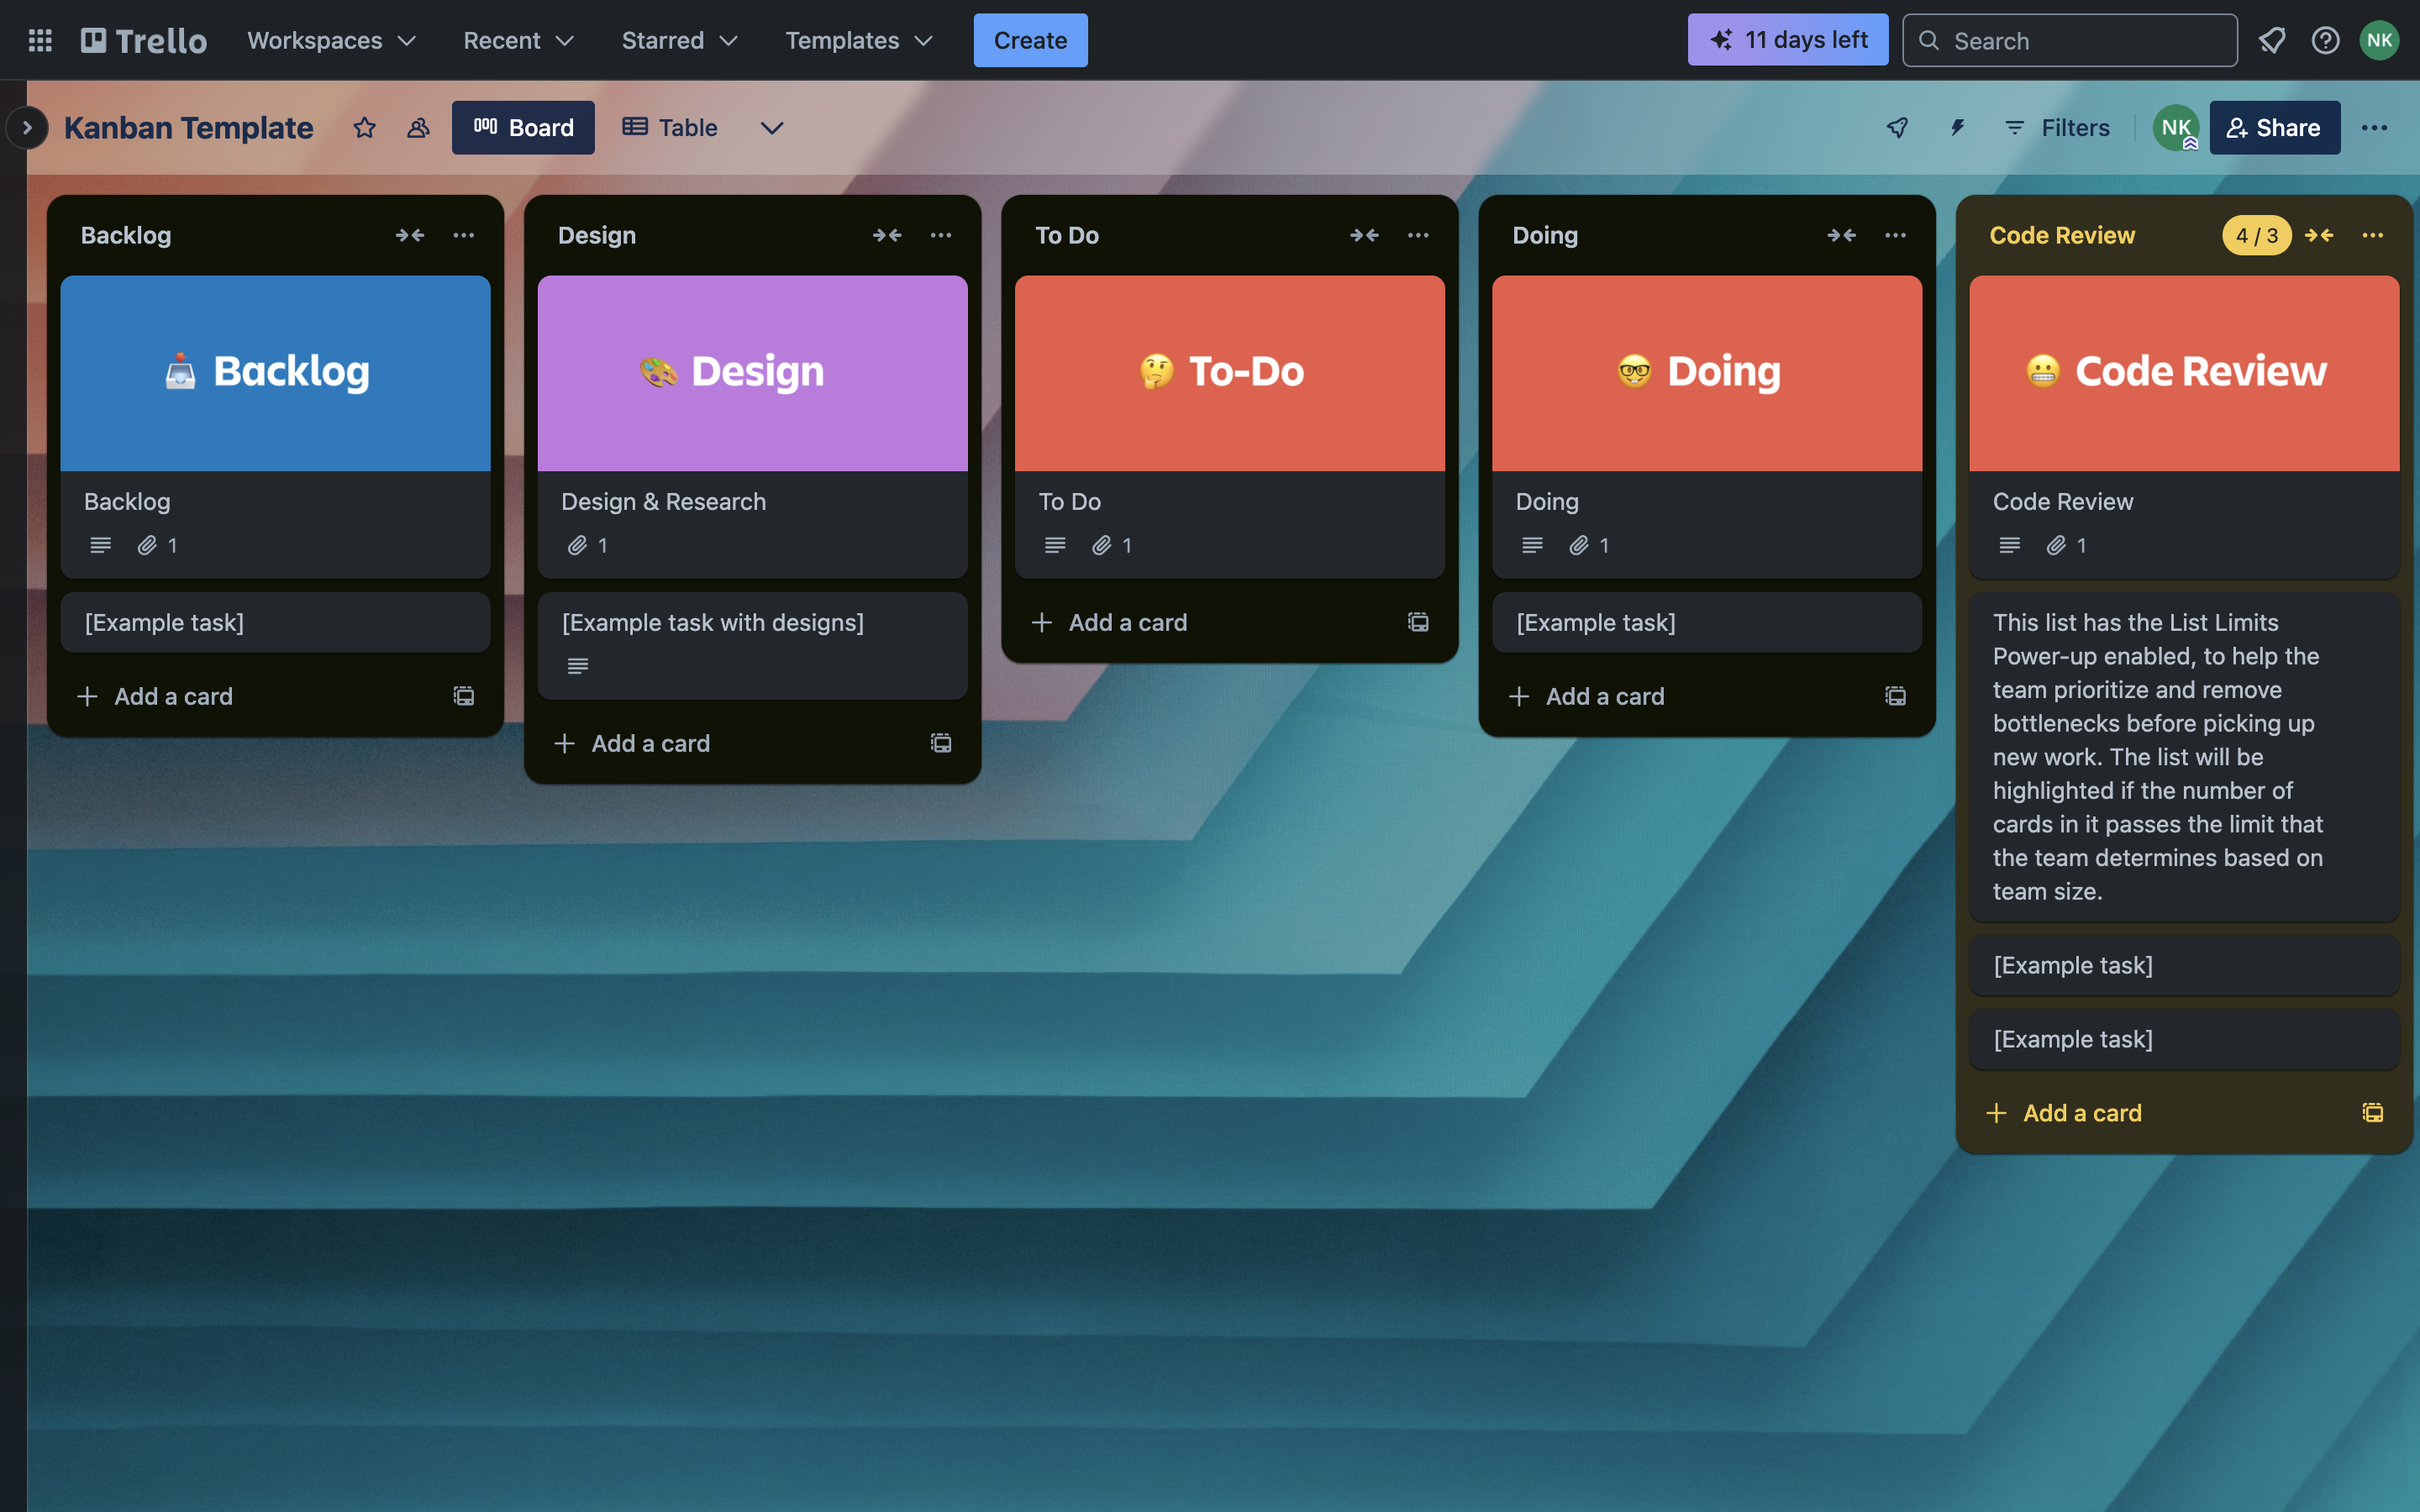
\includegraphics[width=0.6\textwidth]{examples/Trello.png}
            \caption{Trello}
        \end{figure}

        \item \textbf{Asana} \\
        Asana is a tool for managing projects and tasks. Users can create task lists, set deadlines, and track progress. It supports different views like lists, boards, and timelines, making it useful for teams working on complex projects.  

        \begin{figure}[H]
            \centering
            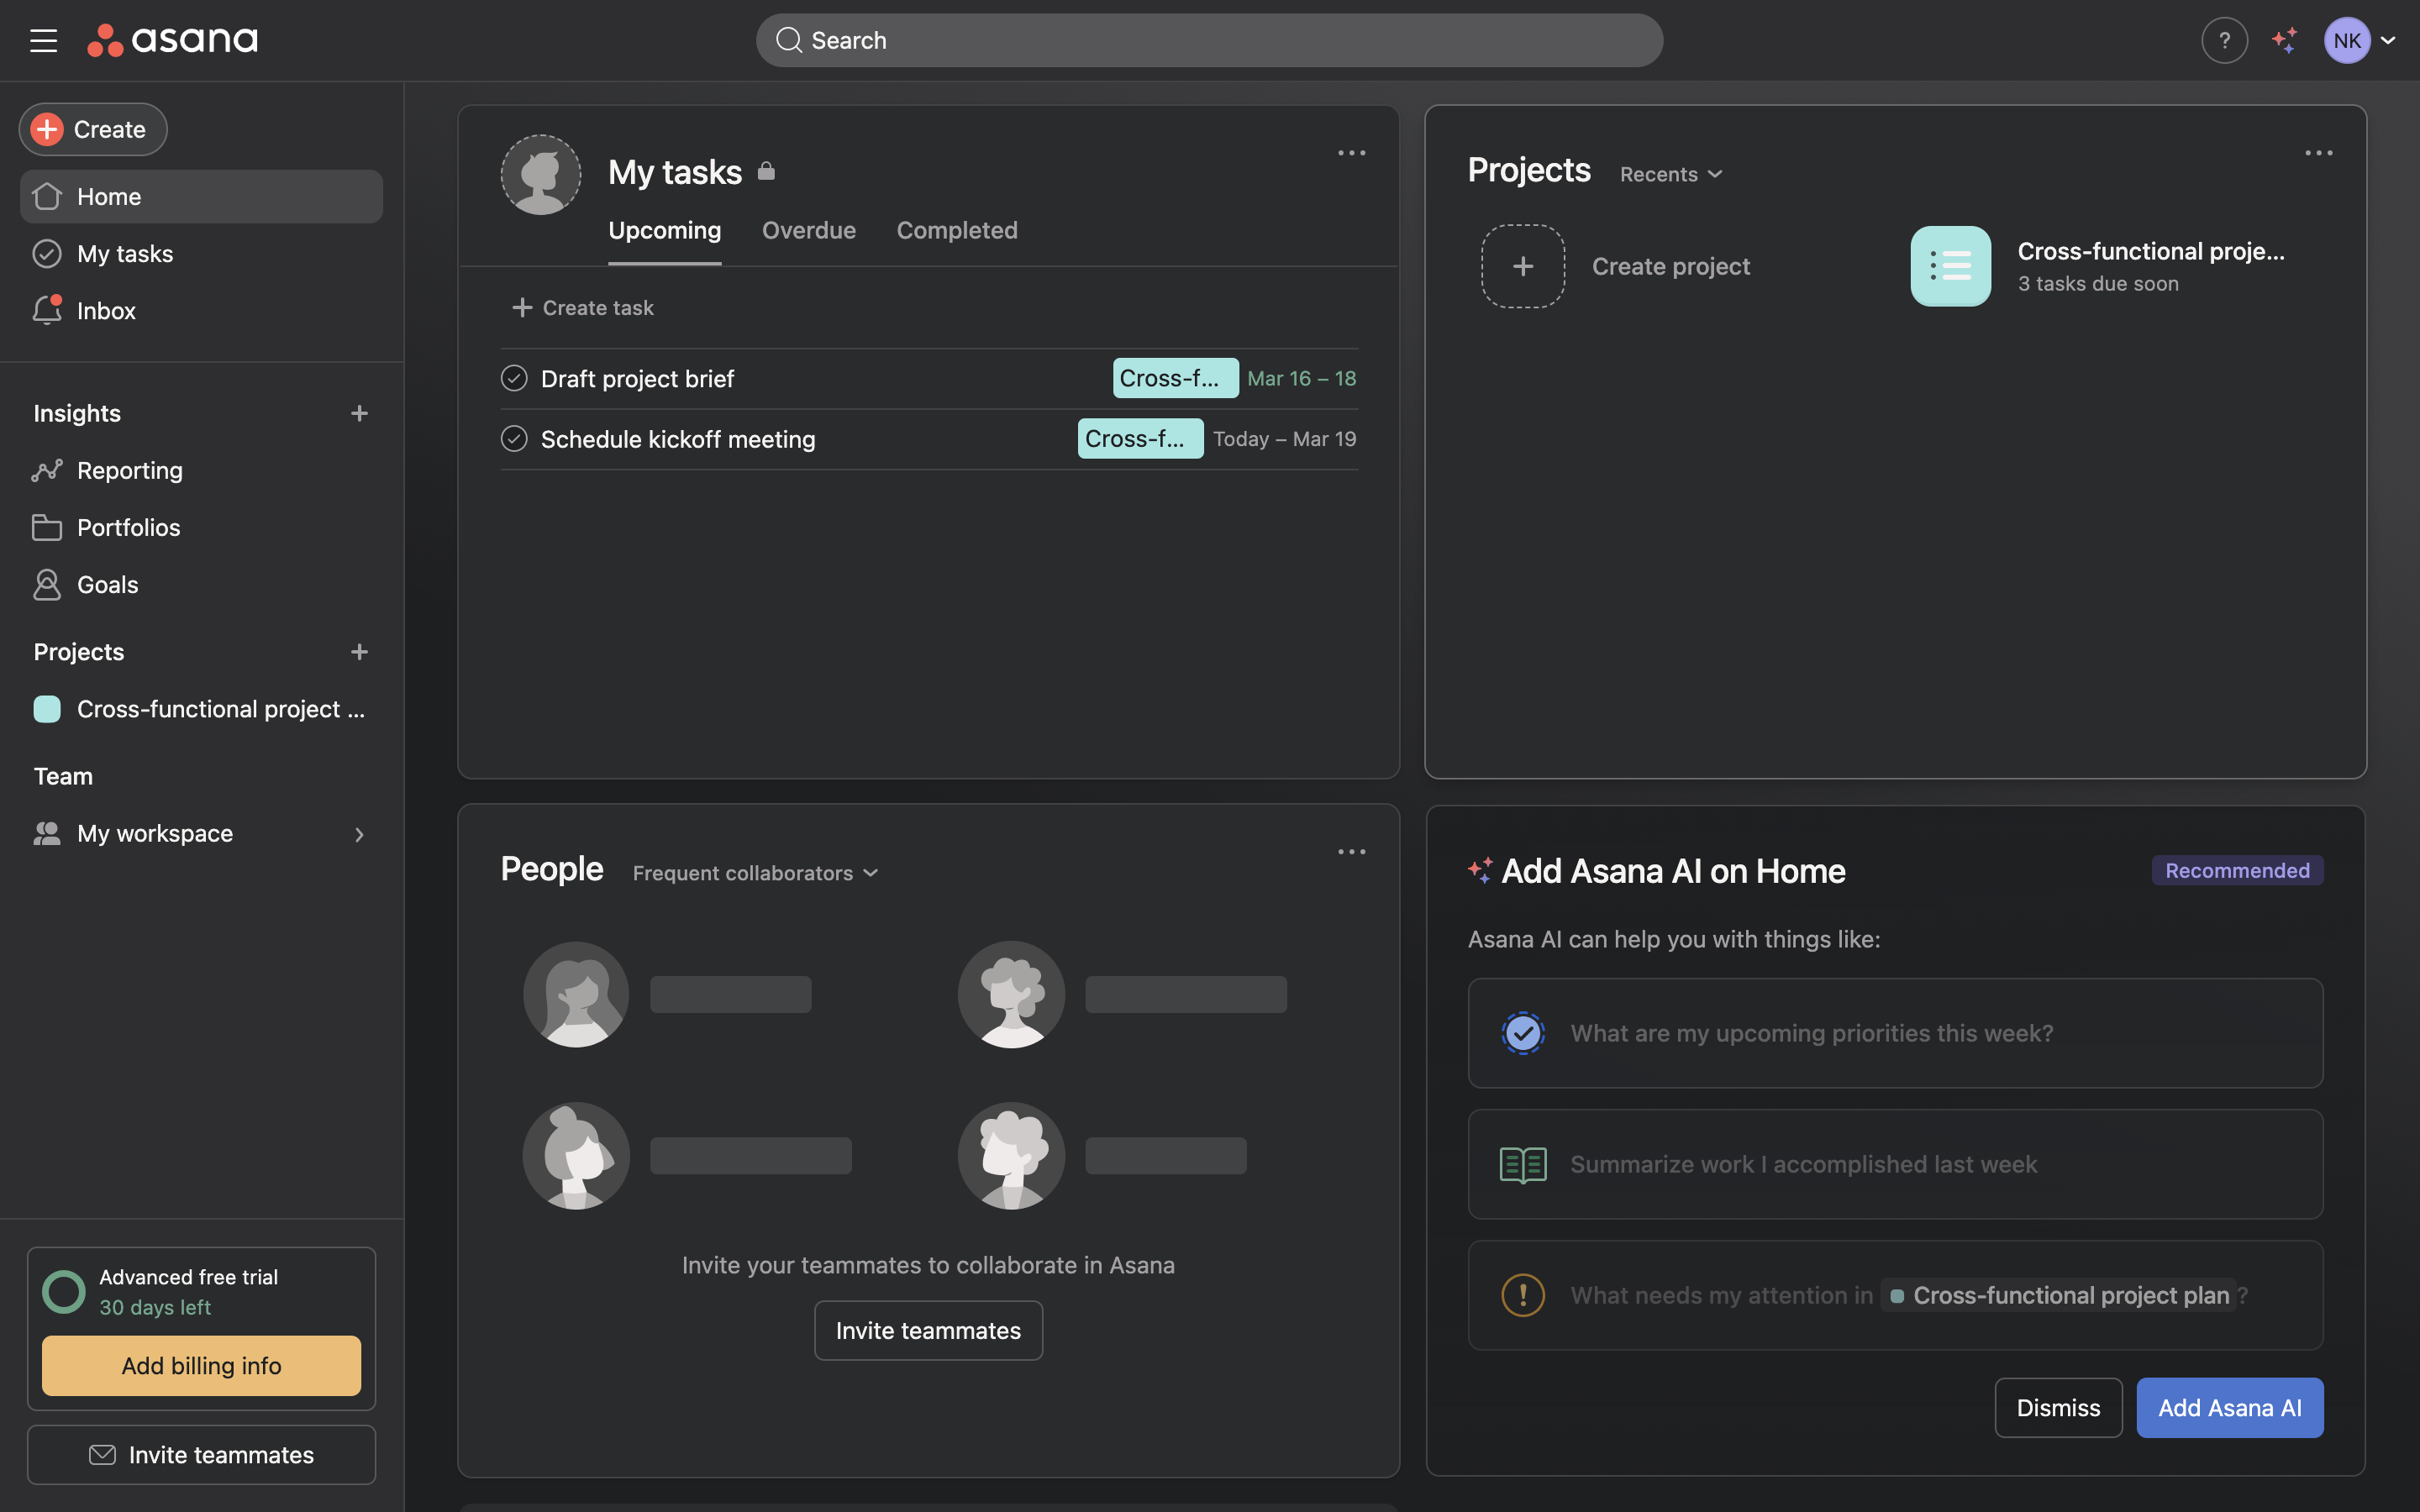
\includegraphics[width=0.6\textwidth]{examples/Asana.png}
            \caption{Asana}
        \end{figure}

        \item \textbf{Monday.com} \\
        Monday.com is a work management tool that helps teams plan and track work. It has customizable workflows, automation, and visual dashboards. Teams can organize tasks in a way that fits their needs.  

        \begin{figure}[H]
            \centering
            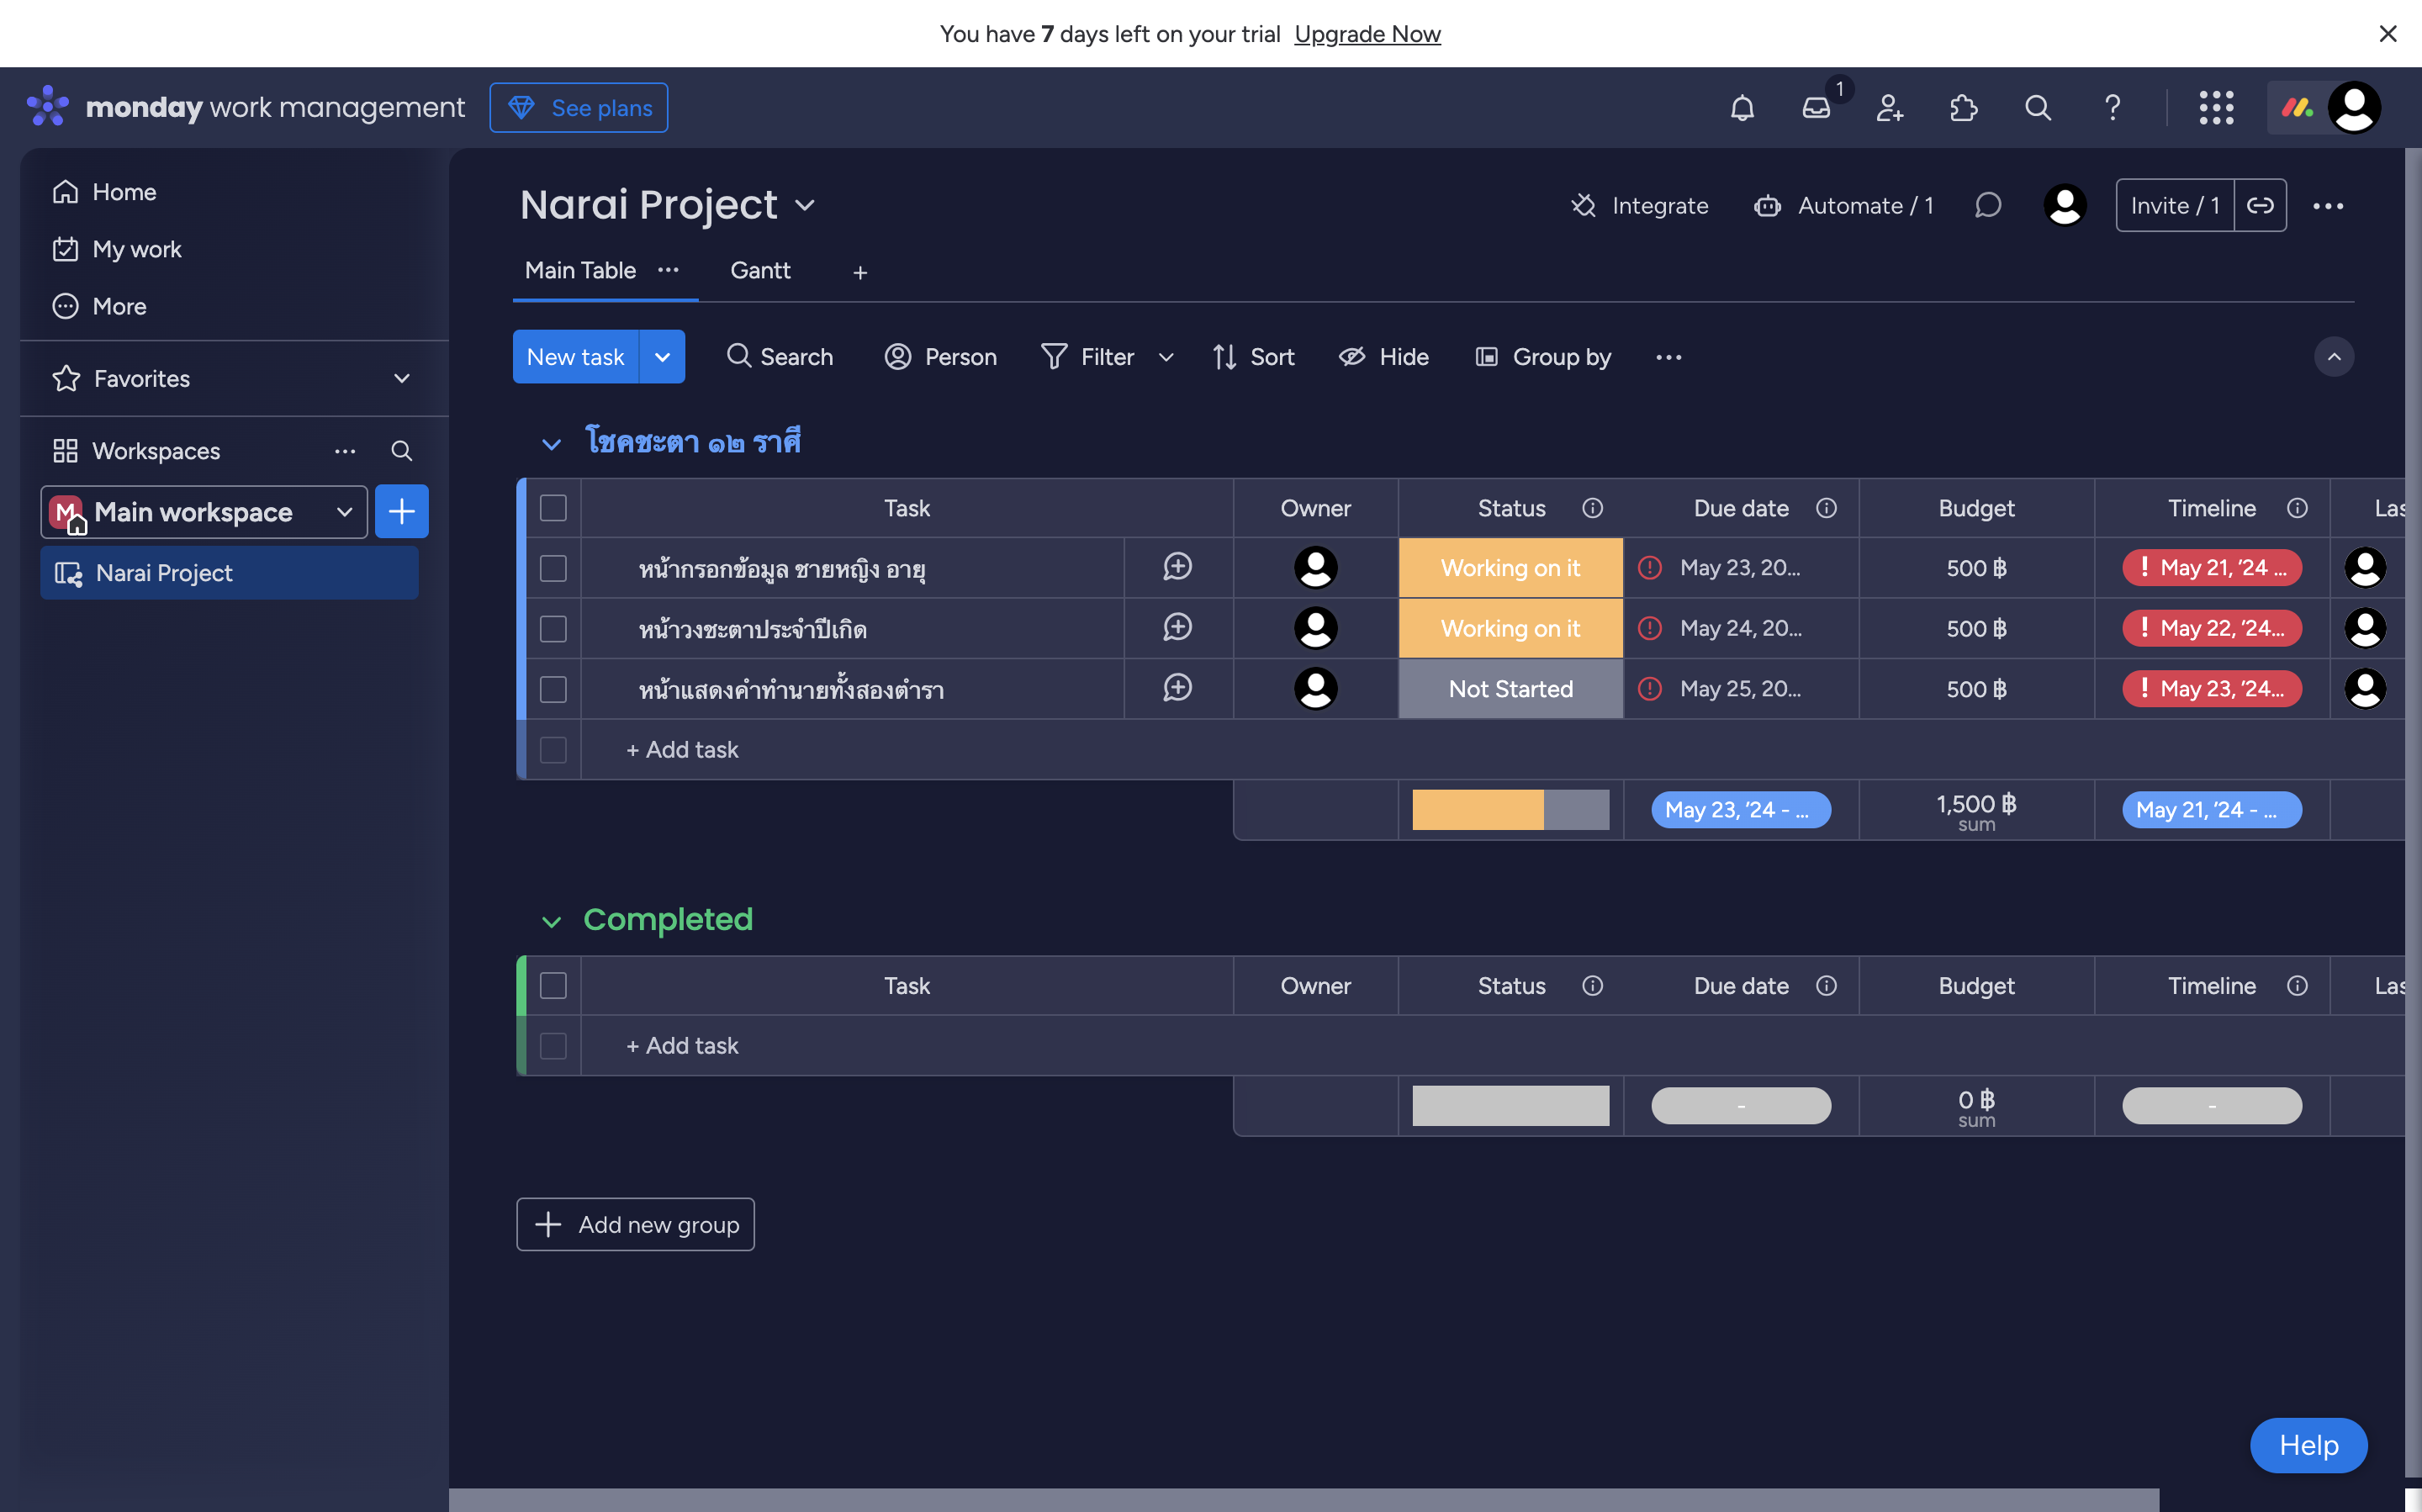
\includegraphics[width=0.6\textwidth]{examples/Monday.png}
            \caption{Monday.com}
    \end{figure}

    \item \textbf{Habitica} \\
    Habitica is a habit tracker that turns daily tasks into a game. Users complete tasks to earn rewards and level up. It makes productivity fun by using game elements to build good habits.  

    \begin{figure}[H]
        \centering
        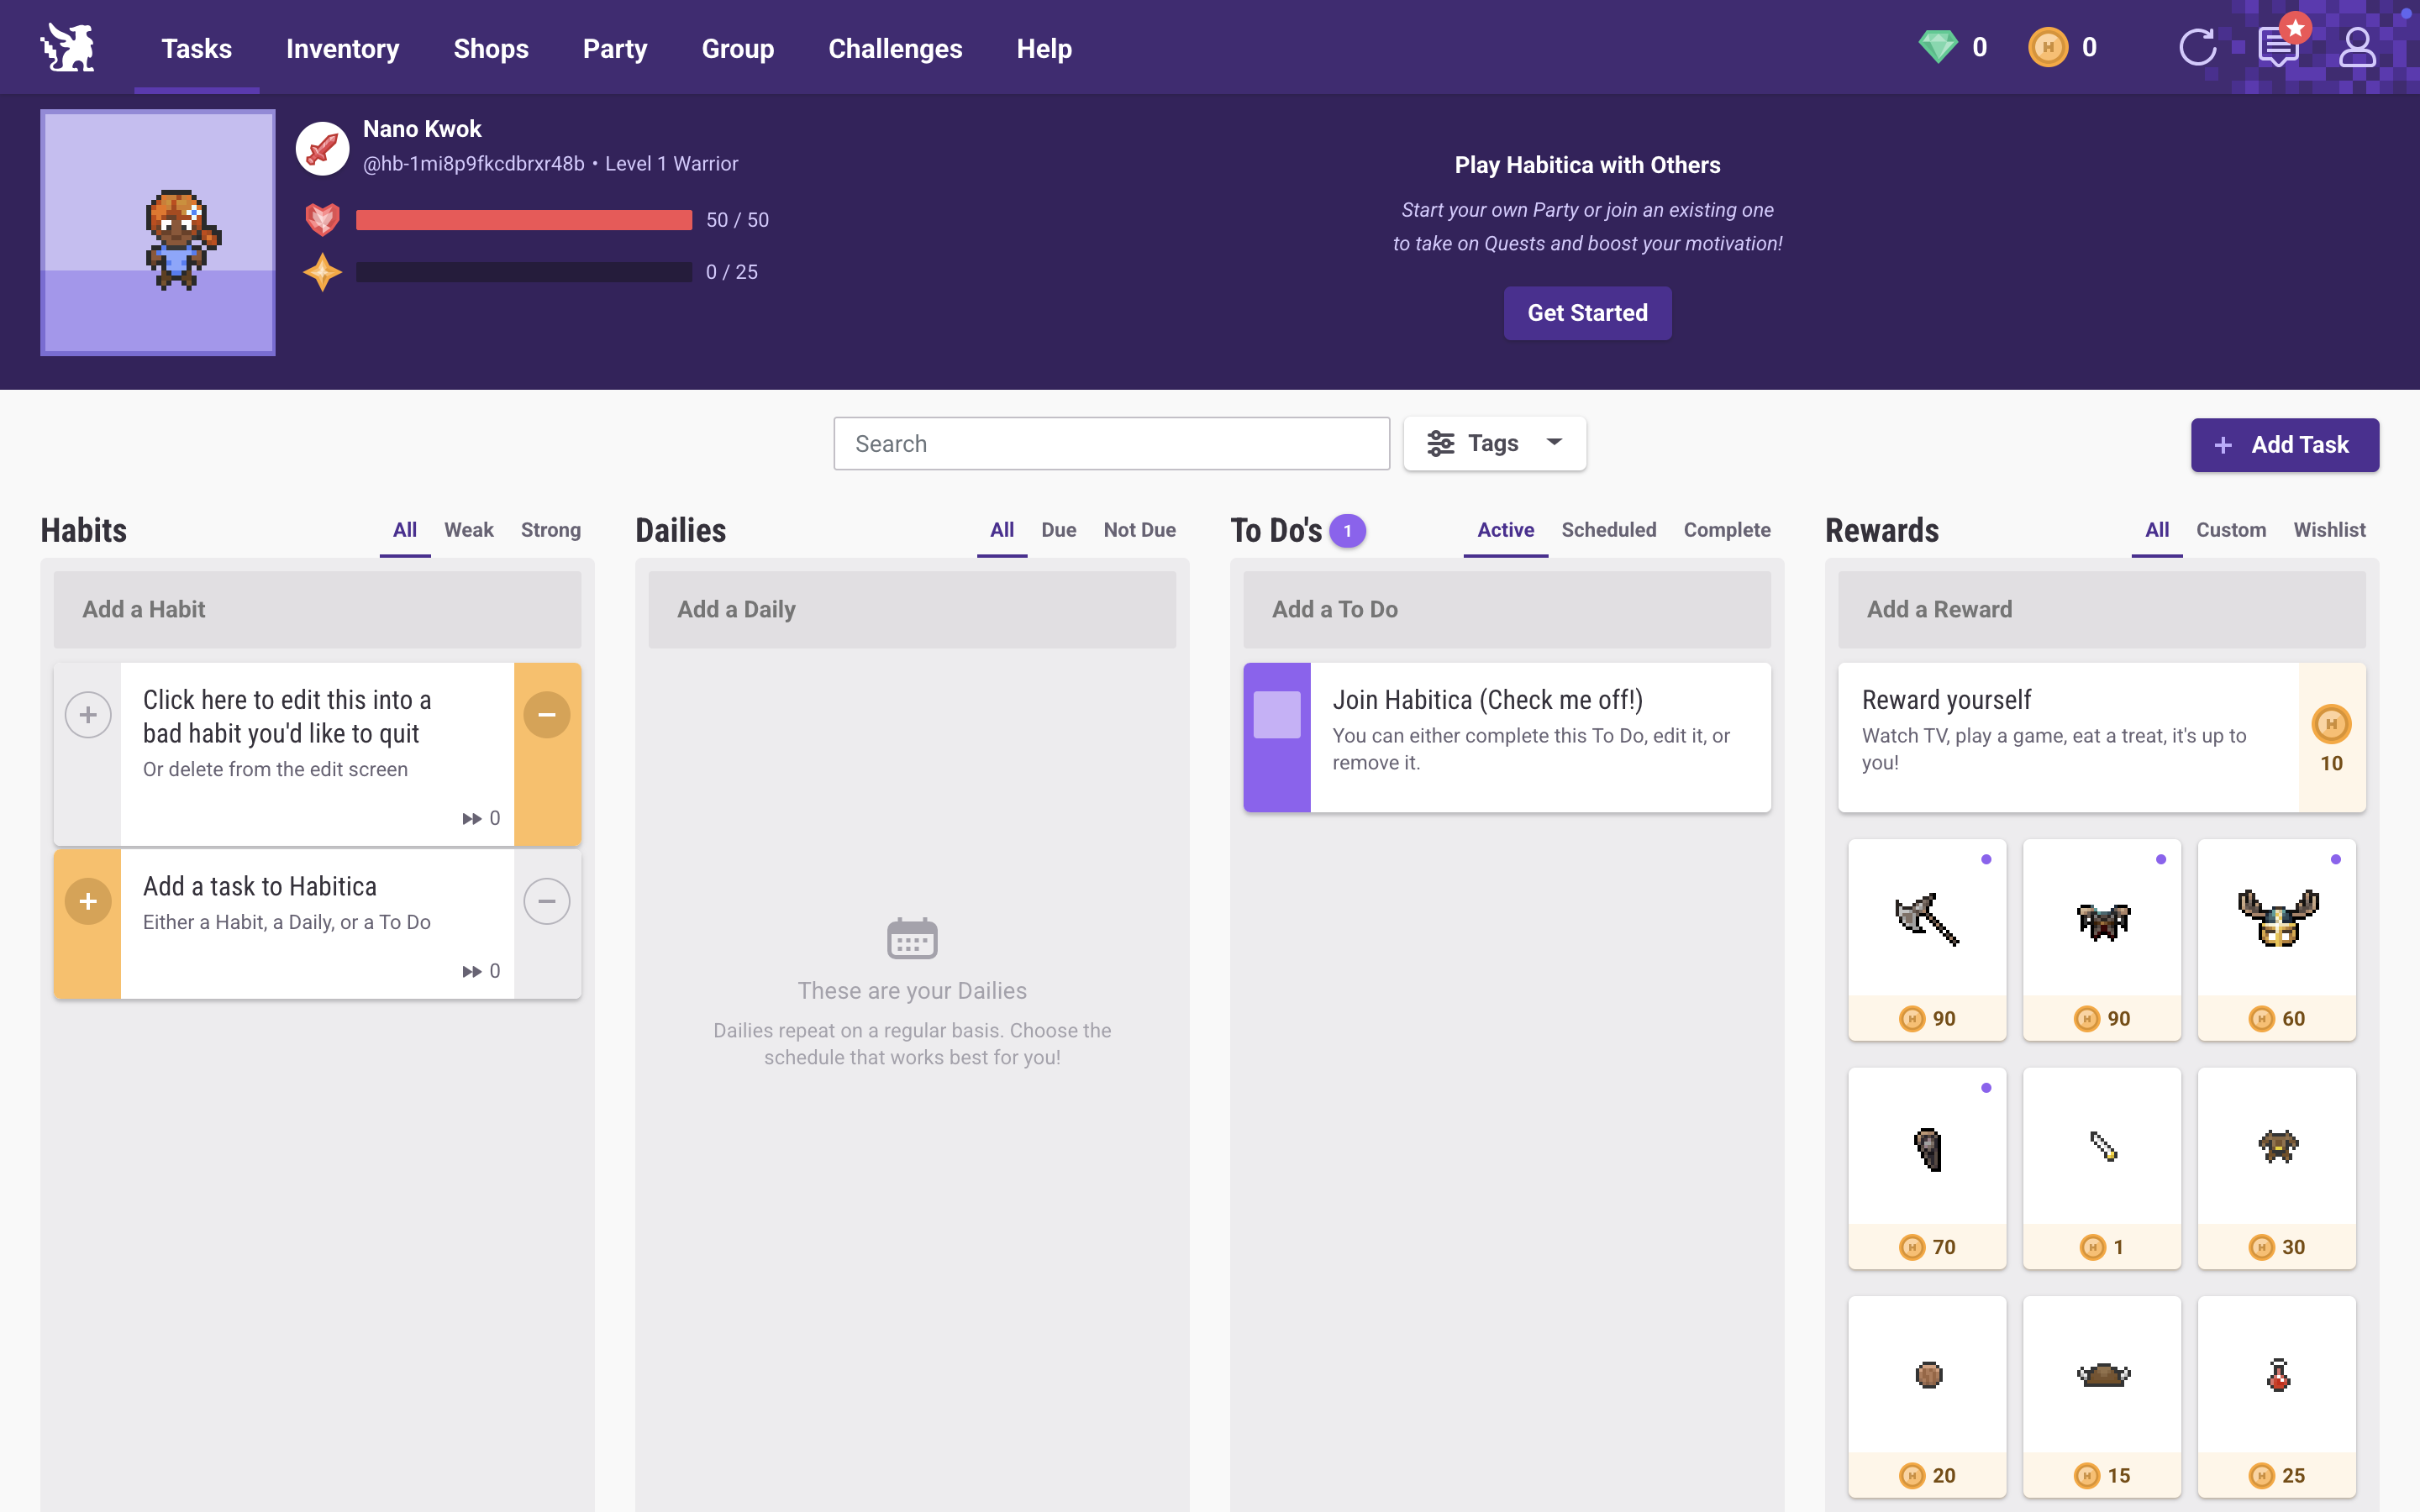
\includegraphics[width=0.6\textwidth]{examples/Habitica.png}
        \caption{Habitica}
    \end{figure}

    \item \textbf{Fucumon} \\
    Fukumon is a gamified productivity app that gives rewards for completing tasks. It helps users stay motivated by making work feel more enjoyable and engaging.  

    \begin{figure}[H]
        \centering
        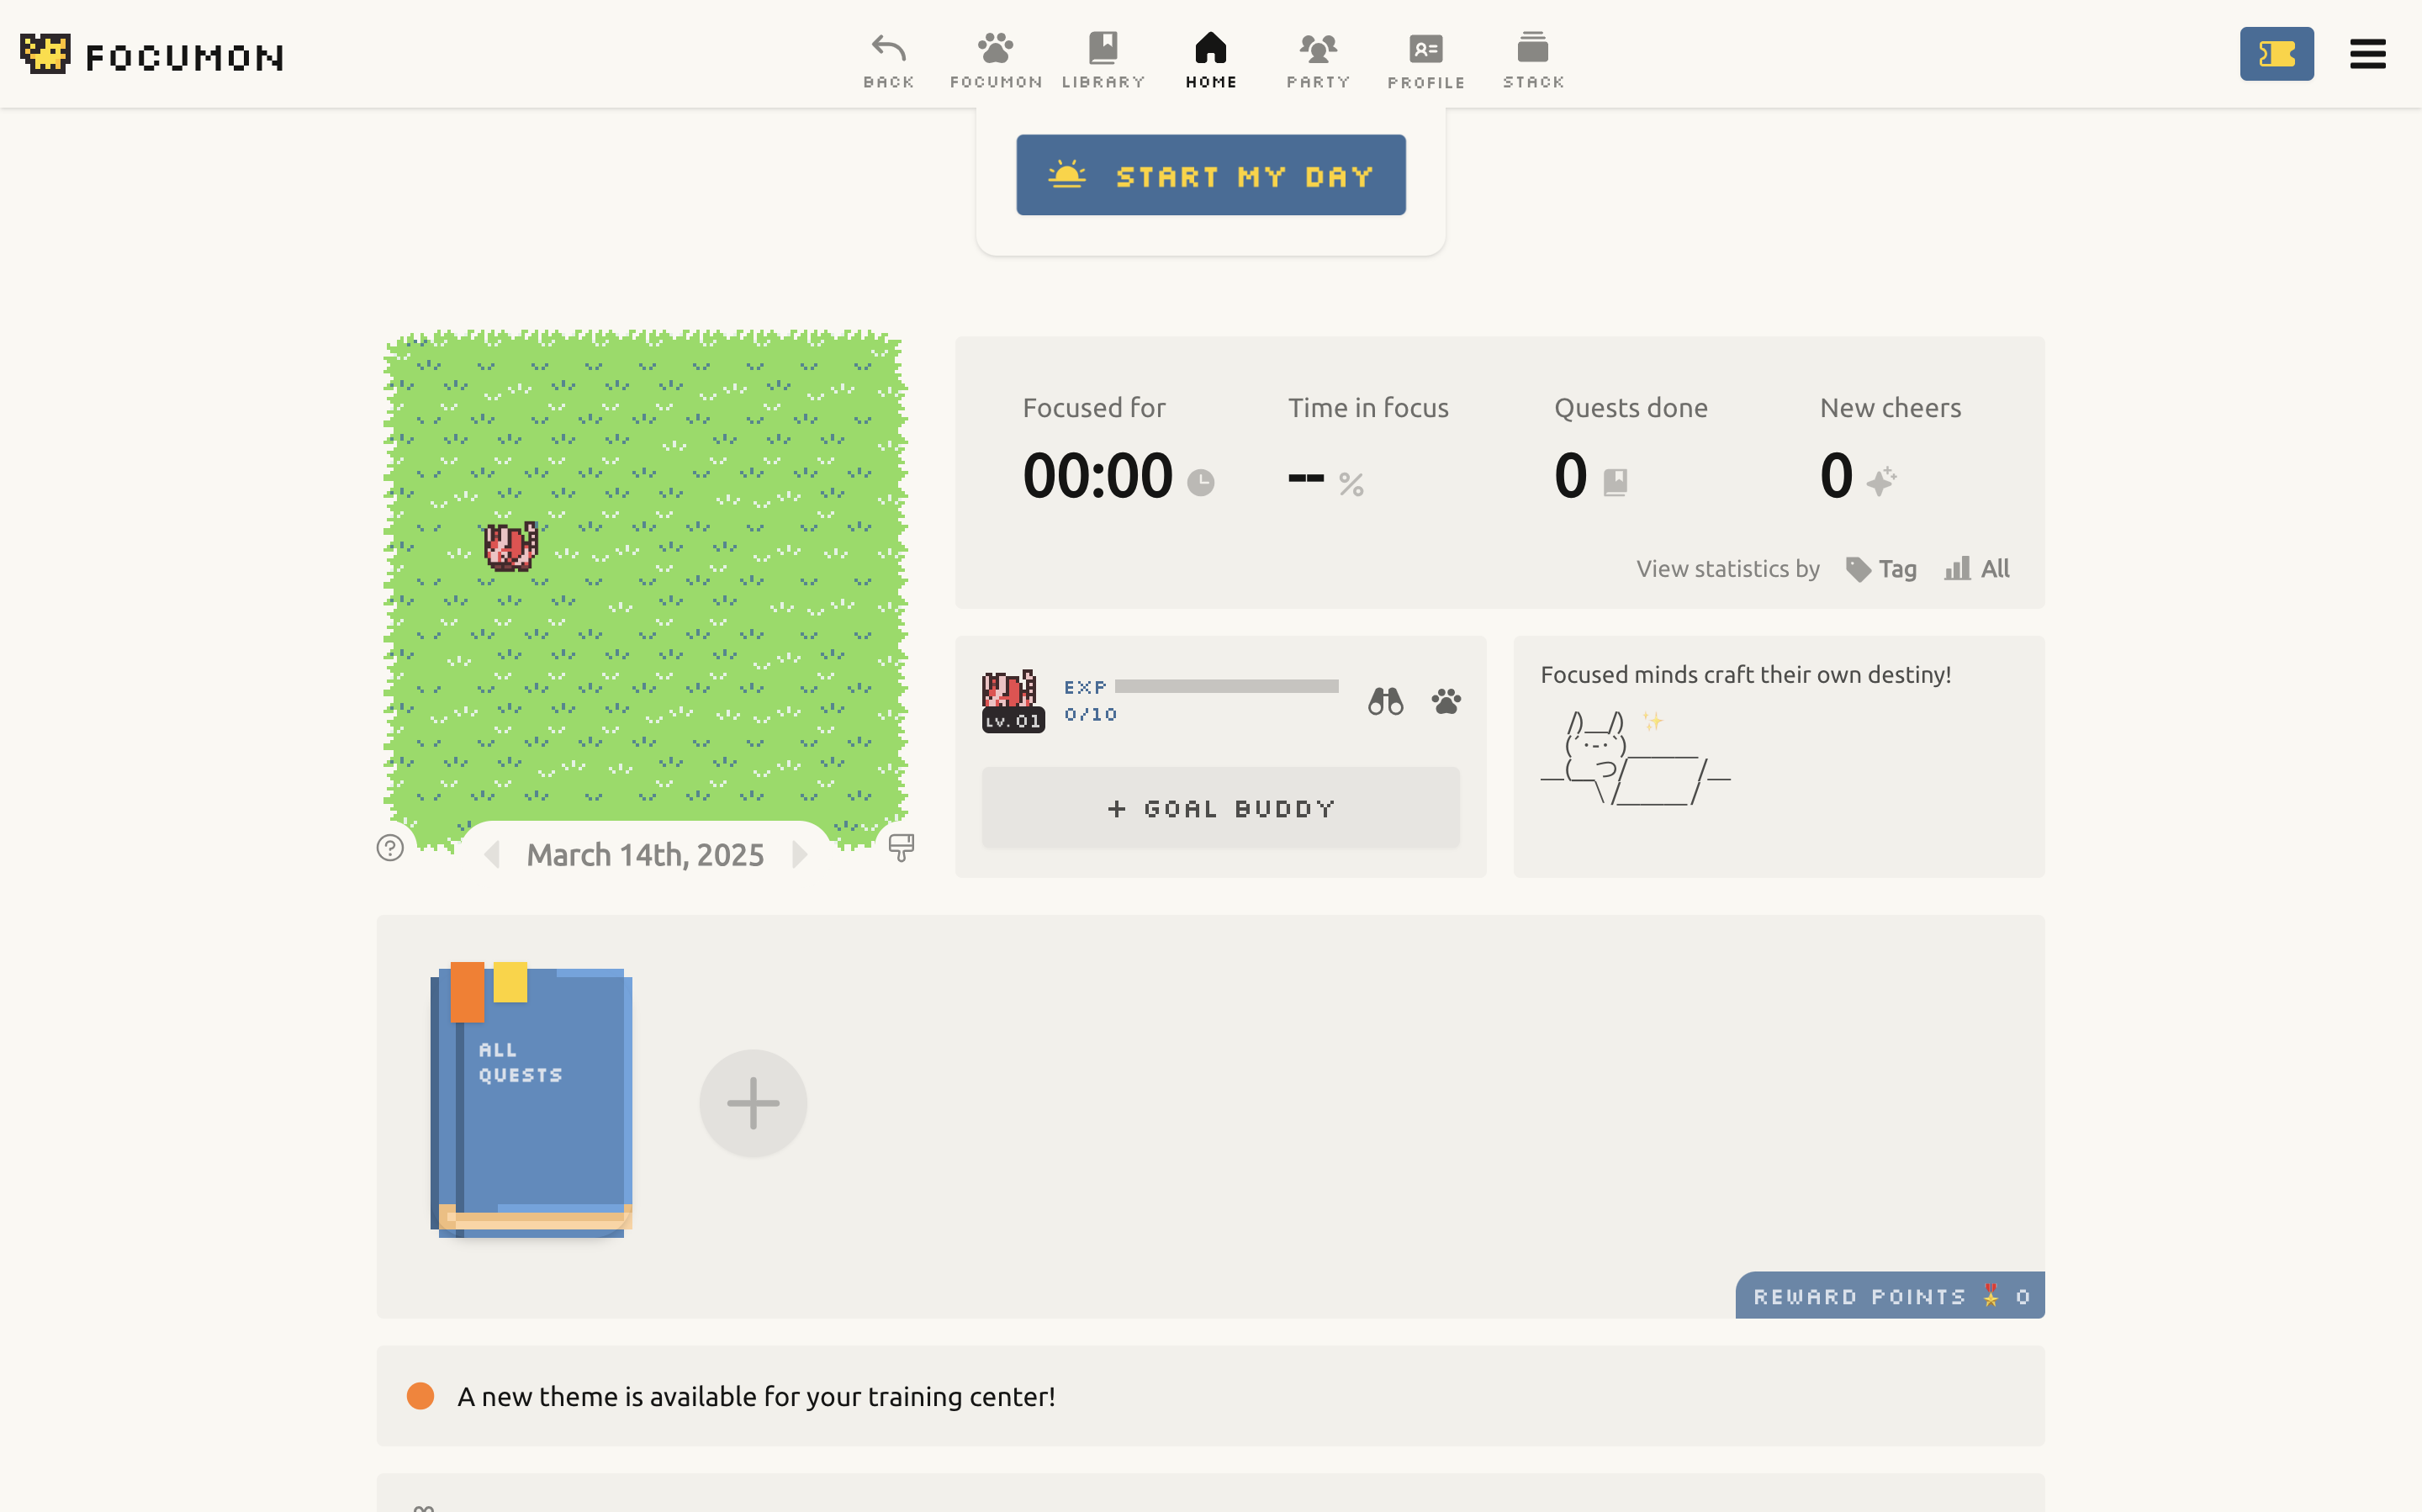
\includegraphics[width=0.6\textwidth]{examples/Fucumon.png}
        \caption{Fukumon}
    \end{figure}   
    \end{enumerate}
    \item \textbf{Product Feature Comparison}

    \medskip
    \noindent\begin{center}
    \begin{table}[ht]
        \centering
        \footnotesize 
        \rowcolors{2}{white}{gray!5}
        \begin{tabularx}{\textwidth}{|X|X|X|X|X|X|X|}        
            \hline
            \rowcolor{gray!70}
            Features & WorkQuest & Trello & Asana & Monday.com & Habitica & Fukumon \\
            \hline
            Task Management & Kanban boards, automation & Kanban boards & Task lists & Custom workflows & Daily tasks & To-do lists \\
            \hline
            Gamification & XP, rewards & No & No & No & RPG-style game & Rewards system \\
            \hline
            AI Feedback & Yes & No & No & No & No & No \\
            \hline
            Collaboration Task assignments & Chat, shared tasks & Boards, comments & Task assignments & Team dashboards & No & Shared tasks \\
            \hline
            Reward System & Leader board, badges & No & No & No & Coins, items & Points, achievements \\
            \hline
            Customization & Workflows, themes & Boards, labels & Templates & Dashboards & No & Task settings \\
            \hline
        \end{tabularx}
        \caption{Feature Comparison Among Competitors}
        \label{tab:feature-comparison}
    \end{table}
    \end{center}
    \medskip

\item \textbf{Product Marketing Comparison}
    \begin{enumerate}
        \item \textbf{Social Media \& Advertising}
        \begin{itemize}
            \item Trello, Asana, and Monday.com focus on business users.
            \item Habitica and Fukumon highlight gamified motivation.
            \item WorkQuest focus on team engagement.
        \end{itemize}
        
        \item \textbf{Website \& Brand Voice}
        \begin{itemize}
            \item Trello and Asana promote workflow efficiency.
            \item Habitica and Fukumon market personal growth.
            \item WorkQuest focuses on gamified collaboration.
        \end{itemize}
    \end{enumerate}

    \item \textbf{SWOT Analysis}
    \begin{enumerate}
        \item \textbf{Strengths}
        \begin{itemize}
            \item Unique gamified approach with AI feedback.
            \item Focuses on team collaboration.
            \item Engaging reward-based mechanics.
        \end{itemize}
        
        \item \textbf{Weaknesses}
        \begin{itemize}
            \item New to the market.
            \item Requires user adaptation to gamification.
        \end{itemize}

        \item \textbf{Opportunities}
        \begin{itemize}
            \item Increasing demand for gamified productivity.
            \item Schools and companies may find it useful.
        \end{itemize}

        \item \textbf{Threats}
        \begin{itemize}
            \item Strong competition from established platforms.
            \item Users may hesitate to switch tools.
        \end{itemize}
    \end{enumerate}

    \item \textbf{Market Positioning}
    \begin{enumerate}
        \item WorkQuest stands at the intersection of gamification and team collaboration.
        \item Differentiates from competitors by integrating AI feedback and engagement.
    \end{enumerate}

\end{enumerate}

% \begin{figure}[h]
%     \centering
%     \includegraphics[width=0.5\textwidth]{examples/asana-competitive-landscape.jpg}
%     \caption{Competitive Landscape by Asana}
% \end{figure}

Refer to an article "How to create a competitive analysis (with
examples)" by Asana. You can use the Competitor Landscape (left image) or
Competitor Analysis Framework (right image) for your project.

\section{Literature Review}
\label{section:literature-review}
    Task management is a critical component of work productivity, yet many teams struggle with disengagement, procrastination, and inefficiencies in collaboration.
    Traditional task management systems often rely on rigid structures that fail to maintain motivation over time. 

    In response to these challenges, gamification has emerged as a promising strategy to enhance engagement and performance. by integrating game-like elements—such as goals, rewards, competition, and collaboration—into workplace settings. Research indicates that gamification can increase work engagement by providing team members with a sense of autonomy, competence, and relatedness, thereby creating a fun and engaging work environment \cite{ncbi:pmc10905147}.
    Additionally, studies have demonstrated practical advantages in several performance metrics resulting from the application of gamification strategies, supported by evidence from real-life case studies. \cite{Employee:Gamification}

    WorkQuest introduces a unique approach to task management by integrating gamification elements—specifically "boss fight" mechanics—and AI performance evaluation. In this system, Users collaborate to complete tasks that weaken and ultimately defeat a boss, adding a layer of strategic engagement. AI-driven analysis provides personalized performance feedback and deadline predictions, ensuring that users receive tailored insights to improve efficiency.
    
\begin{enumerate}
    \item \textbf{Gamification in Task Management} \\
        Gamification, defined as the application of game-design elements and principles in non-game contexts, has emerged as a powerful strategy for enhancing productivity and engagement in working environment \cite{ncbi:pmc10905147} \cite{Employee:Gamification}.
        by incorporating goal-setting for direction, challenges to maintain interest, rewards to reinforce success, and feedback to guide improvement. These elements work together to keep participants engaged, boost performance, and align intrinsic and extrinsic motivations. \cite{Game:Reward}
        
        Numerous studies have demonstrated the benefits of gamification in a variety of contexts. Research by Juho Hamari. (2014) \cite{6758978} reviewed the impact of gamification across sectors and found that its use consistently improved user engagement, productivity, and satisfaction.
        The use of feedback loops, competition, and goal-setting were particularly effective in motivating individuals to perform tasks efficiently

        In the context of task management, gamification has been shown to improve productivity, collaboration, and task completion rates. By incorporating game-like elements, transforms routine tasks into more engaging and motivating activities.
    
        Moreover, gamification has been shown to promote teamwork and collaboration. Deterding et al. (2011) \cite{gamification:designElement} emphasized that gamified systems enhance group dynamics by incorporating features like team challenges, leaderboards, and shared rewards. These elements encourage users to collaborate, share knowledge, and work together towards common goals, ultimately improving collective productivity and communication within organizations
    
        In conclusion, gamification has proven to be an effective method for enhancing productivity in the workplace. By incorporating game elements that align with psychological motivations, gamified systems can increase task engagement, improve collaboration, and ultimately drive higher levels of productivity and performance. However, successful implementation of gamification depends on aligning its features with organizational goals and users preferences.
    \item \textbf{Boss fight mechanics for engagement} \\
        Boss fights in video games are pivotal moments designed to challenge players and heighten engagement. These encounters often require players to utilize all the skills and strategies they've acquired, serving as ultimate tests of their abilities. Successfully overcoming a boss fight provides a strong sense of accomplishment, reinforcing player motivation and progression \cite{toxigon:bossFight}
        
        Emotionally, boss fights take players on a rollercoaster, evoking feelings ranging from excitement and anticipation to frustration and relief. These intense emotional experiences make boss fights memorable and contribute significantly to overall engagement. Additionally, the atmosphere during boss encounters—shaped by music, sound effects, and visual design—enhances immersion, making the battles feel more epic and impactful \cite{toxigon:bossFight}

        Beyond entertainment, the concept of boss fights has also been explored in gamified learning environments. Research suggests that boss fights in educational settings can serve as powerful motivational tools, encouraging students to apply their knowledge and problem-solving skills in high-stakes scenarios. By integrating boss fights into gamified learning, educators can create more engaging and rewarding experiences, similar to how video games challenge and reward players \cite{gamification:Education}
        
        Not only traditional boss fights, we offer a boss collection feature that can further enhance engagement. Rewarding players for defeating bosses and introducing a rotational or exclusive collection system leverages FOMO (Fear of Missing Out) to drive participation. This approach has been successfully used in games like Fortnite and Animal Crossing to sustain player interest and encourage long-term engagement \cite{medium:FOMO}. While some research highlights the potential risks of FOMO in gaming, 
        including compulsive behaviors, when implemented responsibly, it serves as a powerful tool to keep players engaged and invested in the experience.\cite{FOMO:1} \cite{FOMO:2}


    \item \textbf{AI-Driven Personalized Performance Evaluation in collaborate work} \\
        Artificial Intelligence (AI) has transformed performance evaluation by enabling personalized feedback and real-time assessment in collaborative work environments. Unlike traditional evaluation methods, AI-driven systems analyze large datasets to assess individual contributions, track task efficiency, and provide tailored recommendations for improvement. Levy and Williams (2004) emphasize that personalized feedback fosters employee engagement and professional development by addressing specific strengths and weaknesses \cite{Management:SocialContext} Recent advancements in Natural Language Processing (NLP) and Machine Learning (ML) have further refined AI-driven evaluation by enabling contextual understanding and adaptive feedback mechanisms.Research highlight that AI-powered performance tracking improves transparency and fairness by reducing human biases in evaluation process \cite{AI:humanResource}. As organizations increasingly adopt AI-driven performance evaluation, balancing automation with human oversight will be essential to ensure fairness, adaptability, and long-term success in collaborative work environments.

    % \item Reward Systems: Intrinsic vs. Extrinsic Motivation
    
    % \item Kanban Boards and Gamified Task Visualization
    
    \item \textbf{AI-Powered Deadline Prediction and Task Analysis}
    
\end{enumerate}  
Gamification has emerged as a transformative approach to task management, addressing common workplace challenges such as disengagement, procrastination, and inefficiencies in collaboration. By integrating game-like elements—such as goals, rewards, and competition—organizations can foster a more engaging and productive work environment. Research consistently highlights the positive impact of gamification on motivation, teamwork, and overall performance.

The innovative incorporation of boss fight mechanics into task management systems, as seen in WorkQuest, further enhances engagement by introducing challenge-based progression and rewarding collaboration. Drawing from game design principles, boss fights create a sense of accomplishment and urgency, making work tasks more immersive and enjoyable. Additionally, the inclusion of a boss collection feature leverages psychological motivators like FOMO to sustain long-term engagement.

Furthermore, AI-driven performance evaluation provides personalized insights, improving efficiency and fairness in collaborative work. By utilizing machine learning and natural language processing, AI systems offer tailored feedback, mitigate biases, and enhance transparency in performance assessment. However, successful implementation requires balancing automation with human oversight to ensure fairness and adaptability.

Overall, the integration of gamification and AI-driven feedback mechanisms represents a promising evolution in task management. By aligning these strategies with organizational goals and employee preferences, businesses can cultivate a dynamic, motivated, and high-performing workforce.
